\documentclass[tikz,convert={outfile=\jobname.svg}]{standalone}
\usepackage[arrowmos]{circuitikz}
\begin{document}
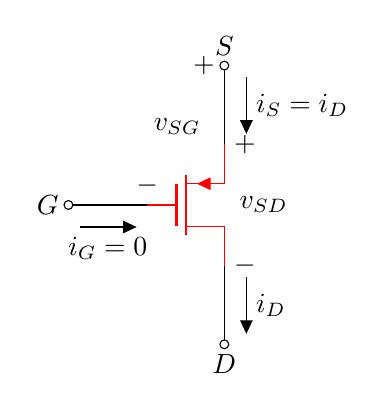
\begin{tikzpicture}
  \draw
  (0, 0) node [pmos, nocircle, color=red] (mosfet) {}
  (mosfet.G)
  node[above] {$-$}
  to[short, -o, f<={$i_G = 0$}] ++(-1, 0)
  node[left] {$G$}
  (mosfet.D)
  node[right] {$-$}
  to[short, -o, f={$i_D$}] ++(0, -1)
  node[below] {$D$}
  (mosfet.S)
  node[right] {$+$}
  to[short, -o, f_<={$i_S = i_D$}] ++(0, 1)
  node[left] {$+$}
  node[above] {$S$}
  (0.5, 0) node[] {$v_{SD}$}
  (-0.6, 1) node[] {$v_{SG}$}
  ;
\end{tikzpicture}
\end{document}
